\chapter{序論}
\label{chap:intro}
\fancyhf{}
\rhead{\thepage}
\lhead{第\ref{chap:intro}章 序論}
\cfoot{\thepage}

本章では,本論文の背景,研究目的および本論文の構成について述べる.


\section{研究の背景}

\subsection{教育の個人最適化と学習科学}
% 導入:学習の個人最適化
近年,教育と情報技術の融合が進む中で,アダプティブラーニングという言葉が注目されている.
個人に最適化された教育の自動提供を実現するもので,その社会的影響の大きさからアメリカを中心として世界的に注目が集まっており,
関連するスタートアップや大学での研究に,多額の資金が投入されている\cite{piccioli2014learning}.

教育を個人に最適化するという考え方は,決して新しいものではない.
現在の学校教育では,一人の教師が複数の生徒に対して同時に教育する形態が一般的であるが,
学習の速度や教科による得手不得手は人それぞれであり,
同じ教育を施しても,十分な理解ができずにつまずいてしまう生徒もいる.
つまずいている生徒に補習を行い,つまずきを克服する手助けをするような,
生徒の学習状態を考慮して教育を設計することは昔から行われてきており,
そうした指導が巧みな教師は「腕のいい」教師として評価されてきた.
しかし,こうした方法では,
習熟の遅い生徒を助けることに重きが置かれるため,習熟が周りより早い生徒への対応は後回しにされることが多く,発展的な学習機会や知的好奇心の向上を妨げることに加え,
現実的な時間と労力を考慮すると,全ての生徒に個別に対応することは困難である.

より個別に教育を受ける手段として,個別指導形式の塾や家庭教師,通信教育なども利用される.
生徒一人一人に教師がつくことで,生徒の習熟度合いを考慮して教育を設計でき,
また能力によって優先されたり後回しにされたりすることもないため,学習内容を個人に最適化するという目的の上ではより望ましい.
しかし,このように教育の粒度を細かくし,個人最適化を進めようとするほど,
教師一人あたりが担当できる生徒の数が減ることによる人材的・金銭的負担や,教師ごとの指導能力の違いなどの問題に直面する.
結局,このような教師のマンパワーに依存した方法では,
誰もが平等に最適な教育を受けるという目的を達成するには,障壁が残る.

すべての生徒に最適な教育を提供するには,
現代の情報技術を活用して,生徒の学習過程を分析し,学習内容を決定するような,新たな教育システムが必要であり,
このようなシステムを作り上げようとする動向は「学習科学」という研究分野として確立され,今日大きな注目を集めている\cite{白水始2014学習科学の新展開}.


\subsection{オンライン教育サービスの普及と学習効果分析の発展}
% 背景1:オンライン学習サービスを利用した個人最適化,データ蓄積に伴う学習効果分析の進展
教育と情報技術の融合の象徴とも言えるアダプティブラーニングの躍進には.
オンライン教育サービスの普及が背景にある.
オンライン教育サービスとは,
学校の教室で一人の教師が複数の生徒に対して同時に授業を行う従来の教育形態と異なり,
PCやモバイル端末を通じて,
オンライン上で提供される学習コンテンツを,生徒が各自で利用するサービスを指す.

オンライン教育サービスの一つであるMassive Open Online Courses(MOOCs)\cite{mcauley2010mooc, pappano2012year,siemens2013massive}は,
多様な分野や難易度の講義から,時間や場所を問わずに,生徒が自分のペースで学習したいものを選択して学習できるというもので,
生徒が自身の習熟度合いに沿った教育を受けられないという問題を解決するプラットフォームとして,活用が期待されている.
例えば,世界最大級のMOOCsの一つであるCoursera\footnote{\url{https://www.coursera.org/}}は,
2017年1月の時点で,
29の国にまたがる148の教育機関とパートナーシップを結び,
コンピュータサイエンス,数学や論理,社会科学などに関する1600以上の講座を,2200万人以上に提供している.
日本では2013年2月に東京大学がCourseraに,2013年5月に京都大学がedX\footnote{\url{https://www.edx.org/}}に参加を表明したことから普及し,
2013年11月には日本版のMOOCsとしてJMOOC\footnote{\url{https://www.jmooc.jp/}}が設立されるなど,
国内外でMOOCsの利用が拡大している.

多様な講座を多くの人に提供するMOOCs以外にも,
より個人の学習過程をサポートすることに特化して設計される
Intelligent Tutoring System(ITS)と呼ばれるオンライン自動学習支援システムの利用も拡大している.
世界最大級のITSであるKnewton\footnote{\url{https://www.knewton.com/}}では,
生徒の学力や理解度と,学ぶべき対象をマッピングすることで、
生徒に最適な学習過程を設計し,
かつ生徒の学習の進捗に応じてその過程を動的に変化させる仕組みを有している\cite{upbin2012knewton}.
近年ではITSとMOOCsの融合も進んでおり\cite{aleven2015beginning},
オンライン教育サービスの利用は世界中で拡大している.

%日本でも,生徒が自宅でオンライン教育サービスを用いて知識を学び,
%学校ではより参加型のディスカッションを行うという「反転学習」の試みが提唱されており,
%オンライン教育サービスが社会に与える影響は今後さらに大きくなっていくといえる\cite{lage2000inverting, 重田勝介2014反転授業}.


% 背景1−B:オンライン教育サービスによるビッグデータの蓄積と活用
さらに,オンライン教育サービスは,新たな学習形態を提供するのみにとどまらず,
これまで困難であった大規模な学習効果分析を可能にするプラットフォームとして期待されている.
オンライン教育サービスでは,
提供された講義を生徒が学習する際に,その学習行動ログをデータとして蓄積することが可能なため,
そうして蓄積された多様な学習者の大規模な学習行動ログから,多様な学習効果の分析が可能になった.
特に,演習問題の回答ログは,その問題が問う知識を学習者が獲得しているか否かを表すため,Knowledge Tracingと呼ばれる知識獲得の分析に利用できる\cite{corbett1994knowledge}.
例えば,生徒の問題回答ログを利用して知識獲得の予測を行った研究\cite{machardy2015toward}は,
世界的に有名なMOOCsの一つであるKhan Academy\footnote{\url{https://www.khanacademy.org/}}に蓄積された100万件以上の問題回答ログを使用しており,
教育の分野における大規模な学習効果分析の一つである.
生徒が個人で利用するというオンライン教育サービスならではの特性によって,
このような研究成果を元に最適化された学習コンテンツを,個人に提供することが容易になったため,
教育の個人最適化を進める動きは,急速に活発化している.


\subsection{深層学習の躍進と知識獲得予測}
% 背景2:深層学習の高まり
一方,近年,教育に限らない多くの研究領域で,深層学習が注目されている.
従来の機械学習では,人間が問題の特徴を捉えて素性を設計する必要があったが,
深層学習では,目的に応じた素性を,データから自動で学習することが可能になり,
画像認識\cite{schroff2015facenet,szegedy2014going},
音声認識\cite{hinton2012deep, bahdanau2015end},
機械翻訳\cite{sutskever2014sequence, dong2015multi}等,
多様な研究領域で飛躍的な進展が報告がされている.
直近の一年間では,
画像から動画を生成する研究\cite{vondrick2016generating}や,
会話を人間と同程度に認識できるとする音声認識の研究\cite{xiong2016achieving},
一部の欧米言語間の文レベルで,ほぼ人間と同等に正確な翻訳を実現したとする機械翻訳の研究\cite{wu2016google}なども報告されており,
深層学習によって,日々驚異的な成果が生み出されている.
また,2016年3月に人間のプロを倒したことで一躍有名になった,Google Deep Mindが開発したコンピュータ囲碁プログラムの「AlphaGo」\cite{silver2016mastering}は,
過去の人間の対局の記録である棋譜から,深層学習によって人間の囲碁の打ち方を学習し,自己対局による強化学習を通して,
今後10年は不可能と言われていた,人間のプロを打ち負かすほどの棋力を獲得した.
AlphaGoは,単に人間の打ち方を真似ただけでなく,
それまで人間が考えつかなかったような斬新な手を学習しており,囲碁界に衝撃を与えている.
このように,深層学習は,人間が認識できないようなデータの複雑な特徴を捉えることで,
これまで人間が作り上げてきた概念を,大きく塗り替える可能性を秘めている.


こうした深層学習の技術は,学習効果の分析にも活用が期待されている.
特に,オンライン教育サービスの普及によって盛んになった知識獲得予測の研究も,深層学習の適用によって大きく進展した.
Piechらが発表した,知識獲得予測に深層学習を活用するDeep Knowledge Tracing(以下,DKT)という手法では,
時系列分析でよく用いられる深層学習モデルであるRecurrent Neural Networks\cite{williams1989learning}を活用することで,
高い性能で知識獲得を予測できること,
また,予測モデルを分析することで知識間の関係性をネットワークとして抽出できることが報告されている\cite{piech2015deep}.


\subsection{知識獲得予測の問題点}

しかし,こうした知識獲得予測に深層学習を適用するDKTの研究においても,ある問題が存在する.
知識獲得を予測するアルゴリズムの部分には深層学習を適用しているものの,
素性となる「知識」は,事前に人間が作成した知識分類によって定義されており,
人間が設計した素性を利用するという旧来の状況から脱していない.
人間が作成した知識分類というのは,
「知識の体系はこうなっているはずだ」ないしは「この体系に基づいて教える・教えられることが望ましい」という専門家の仮説や理論に基づいて作られたものである.
そのため,人間にとっての可読性は高いとしても,
実際の生徒の学習過程を定量的に分析した結果を反映し,知識獲得を予測する上で最適化された分類であるという根拠はない.
今日多様な分野で成果を生んでいる,データから特徴を自動で学習できる深層学習を活用すれば,
人間が認識できないような,人間の学習過程に潜む複雑な知識構造を反映した,予測を最適化するような知識分類を学習できる可能性は高く,
生徒の学習効率を最適化するという最終的な目標を真に達成するには,
知識分類自体も深層学習によって最適化される必要があるといえる.


以上の問題意識に基づいた,既存研究との本研究の差分のイメージを図\ref{fig:problem}に示す.
\begin{figure}[htb]
\begin{center}
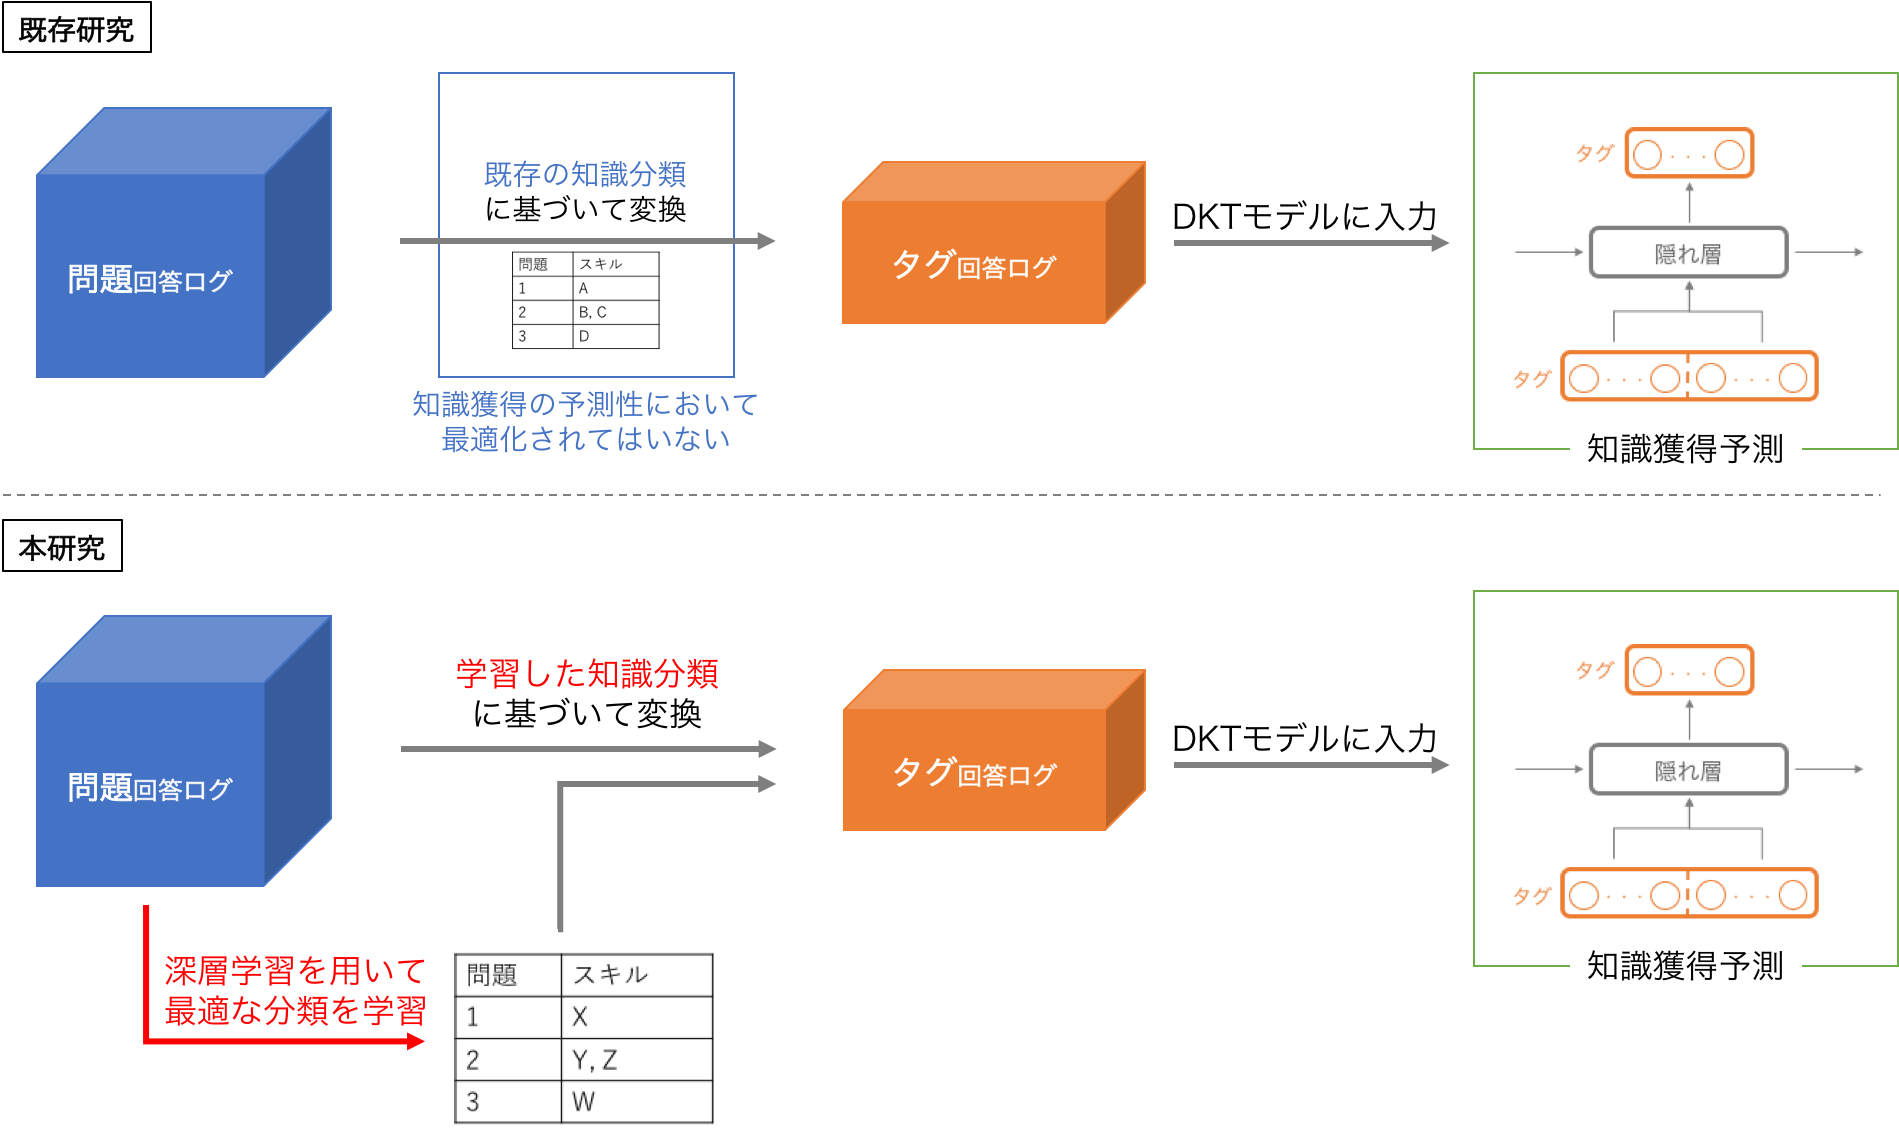
\includegraphics[width=400pt]{./img/problem3.png}
\end{center}
\caption{既存研究と本研究の差分のイメージ}
\label{fig:problem}
\end{figure}


\vvspace
以上,本研究の背景について述べた.

次に,本研究の目的について説明する.


\section{研究の目的}
本研究では,
現在の知識獲得予測に用いられている,人間が作成した知識分類は,人間の知識獲得の予測を行う上では最適化された表現ではない,という仮定に立ち,
下記を検証することを目的とする.
\vvspace
深層学習によって抽出した知識分類を用いることで,人間が作成した知識分類を用いる場合よりも,高い精度で知識獲得予測を行うことができる.
\vvspace
%\begin{itemize}
%\item 深層学習によって抽出した知識分類を用いることで,専門家が作成した知識分類を用いる場合よりも,高い精度で知識獲得予測を行うことができる.
%\end{itemize}

本論文では,人間が作成した知識分類を所与のものとせずに,
問題の回答ログデータのみを深層学習に適用し,回答正誤予測を行う過程で,
その予測性を最適化する知識分類を抽出することを目的としている.
従来,専門家が事前に分類することが必要であった問題コンテンツの集合から,
知識獲得の予測性を最適化する知識分類を,深層学習によって自動で抽出できることを明らかにすることは,
既存の学問体系やカリキュラム設計の再構築につながるだけでなく,
人間の知識状態の推移するメカニズムを解明することにもつながり,
学術的な意義が大きいと考える.


\vvspace
以上,本研究の目的について述べた.

次に,背景と目的を踏まえて本論文の構成について述べる.



\section{本論文の構成}
以降の本論文の構成について述べる.

\vvspace

2章では,関連研究について述べる.
知識獲得予測の関連研究を俯瞰し,
周辺概念を整理することで,本研究の学術的位置づけを明確にする.

\vvspace

3章では,分析手法について述べる.
まず,生徒の回答正誤を予測する過程で最適な知識分類を学習する手法について説明し,
また,その結果から抽出された知識分類を分析する手法について説明する.

\vvspace

4章では,
実験で用いるデータセットについて述べる.
オンライン教育サービスにおける生徒の学習回答ログである,2つのデータセットを紹介し,
本研究に適用するための事前の処理を説明する.

\vvspace

5章では,実験について述べる.
本研究で行う実験を大きく3つに分け,各実験の設定を述べた後,
実験結果について述べる.
実験結果においては,
提案手法によって抽出された知識分類を用いることで,既存の知識分類を用いた場合よりも高い精度で知識獲得を予測できることを示し,
予測性を最適化する知識分類が抽出されたことを定量的に確認する.
さらに,抽出された知識分類を既存の知識分類と定量的・定性的に比較することで,その性質を解釈する.

\vvspace

6章では,実験結果を踏まえた考察を述べる.
まず,本研究で用いた手法や抽出された知識分類について,
実験結果を踏まえて,その性質を考察し,実際の教育現場への適用法について述べる.
また,
本研究で用いた分析手法の,多様なデータへの適用可能性について議論し,
教科によらず適用できる可能性があること,教科によって抽出される知識分類の性質が異なる可能性があること,
一方で,複合的な学問や専門性の高い学問については,適用可能性の検証実験が必要であることを述べる.
さらに,
本研究で抽出された知識分類を離散表現に改めることの重要性や可能性について論じ,
また,本研究で用いた分析手法が,教育学以外の分野にも応用できる可能性を持つことを論じる.

\vvspace

最後に,7章で結論を述べる.



\vvspace
以上,序論について述べた.
次に,関連研究について述べる.


